\subsection{Die Braggsche Gleichung}
Die Braggsche Gleichung, welche eine Bedingung f�r konstruktive Interferenz bei der elastischen Streuung von Photonen an einem Kristallgitter liefert, wurde 1913 von H. Bragg und W. L. Bragg aufgestellt. Sie ist einfacher als die Beschreibung von Max von Laue, welcher die Beugung von R�ntgenstrahlen an Kristallen unter schw�cheren Voraussetzungen dargestellt hat. Aufgrund deren �quivalenz wird meistens die Braggsche Gleichung bevorzugt.
Die Folgende Graphik veranschaulicht den Strahlengang und erkl�rt die Braggsche Gleichung gleichzeitig:
 \begin{figure}[H]
 	\centering
   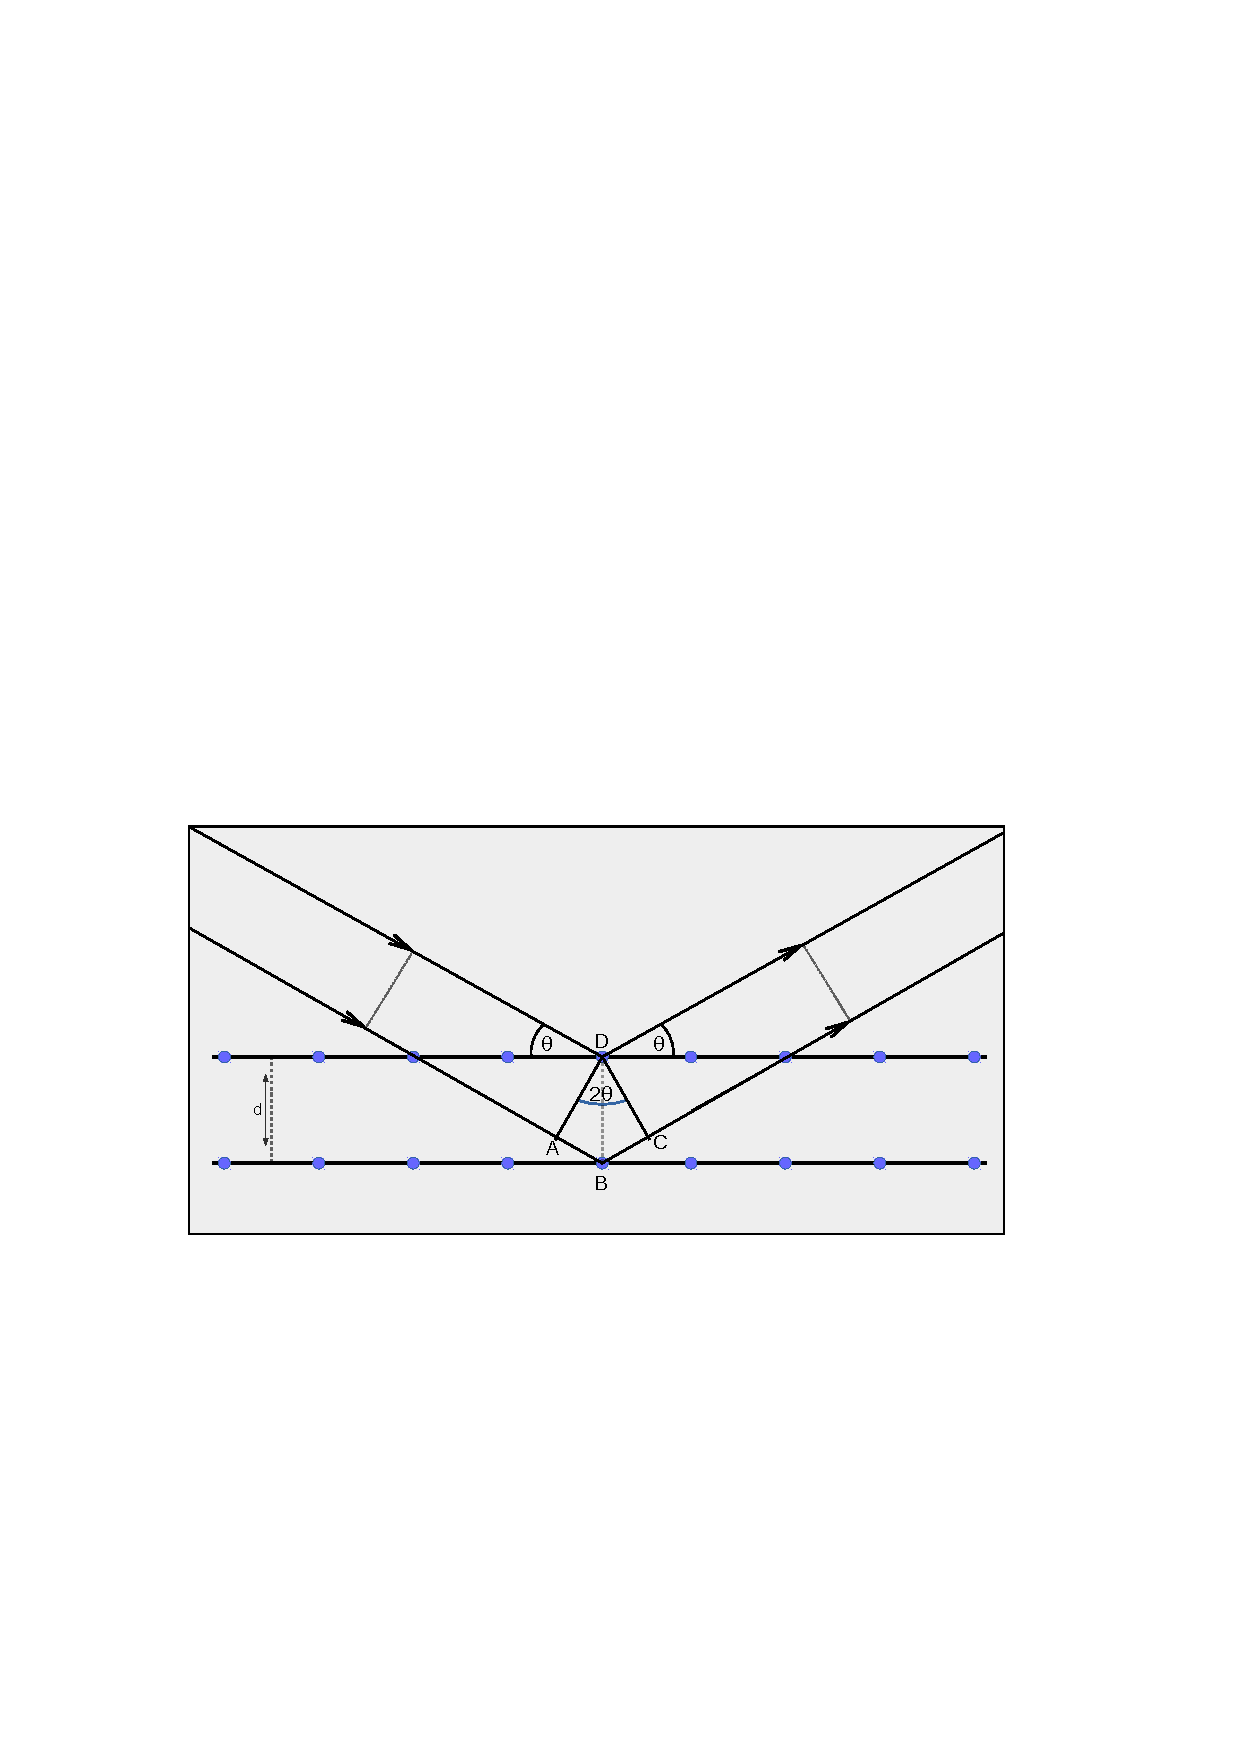
\includegraphics[scale=1, clip = true, trim = 2cm 8.8cm 2cm 14cm]{Bragg.pdf}
 	\caption{Braggsches Beugungsbild}
 	\label{fig:Bragg}
 \end{figure}
Wie man unschwer an Abb. \ref{fig:Bragg} abliest, ist die Bedingung f�r konstruktive Interferenz\footnote{Wobei die Ordnung des Reflexes �blicherweise in die Millerindizes eingeht}:
\begin{align}
\lambda = 2 d_{[nh,nk,nl]} \sin{\Theta}
\end{align}
